
\documentclass[12pt]{article}
\usepackage[russian,english]{babel}
\usepackage[backend=biber,style=numeric,sorting=none]{biblatex}
\usepackage{csquotes}
\addbibresource{sources.bib} %% подключение библиографической базы из файла sample.bib
\usepackage{fontspec}
\usepackage{listings}
\usepackage{url}
\usepackage[dvips]{graphicx} %вставка графики
\graphicspath{{images/}}%путь к рисункам
 \usepackage[a4paper,top=2cm,bottom=2cm,left=3cm,right=3cm,marginparwidth=1.75cm]{geometry}
\usepackage{ctable}
\setmainfont{Times New Roman}
\usepackage{amsmath}

\bibliography{sources.bib}

\lstdefinestyle{C}{               
    numbers=left,
    numbersep=10pt,
    breaklines=true
}
\begin{document}
\begin{titlepage}
\begin{figure}
    \begin{center}
        
\includegraphics[width=0.06\textwidth]{img/znachok_dvfu.png}
    \end{center}
\end{figure}
\thispagestyle{empty}

\begin{small}

\renewcommand{\baselinestretch}{2.0} % Полуторный интервал
\centerline{\large{МИНИСТЕРСТВО НАУКИ И ВЫСШЕГО ОБРАЗОВАНИЯ РОССИЙСКОЙ}}
\centerline{\large{ФЕДЕРАЦИИ}}
\centerline{Федеральное государственное автономное образовательное учреждение}
\centerline{высшего образования}
\centerline{\textbf{«Дальневосточный федеральный университет»}}
\centerline{\textbf{(ДВФУ)}}

\noindent\rule{\textwidth}{4pt}
\specialrule{.1em}{.05em}{.05em}

\centerline{\textbf{ИНСТИТУТ МАТЕМАТИКИ И КОМПЬЮТЕРНЫХ ТЕХНОЛОГИЙ}}
\centerline{\textbf{Департамент математического и компьютерного моделирования}}

\vfill

\vfill

\centerline{\textbf{Реферат}}
\centerline{\textbf{о практическом задание по дисциплине АИСД}}
\centerline{«Алгоритм поиска D*Lite»}
\par\noindent\rule{\textwidth}{0.3pt}
\centerline{направление подготовки 09.03.03 «Прикладная информатика»}
\centerline{профиль «Прикладная информатика в компьютерном дизайне»}

\vfill

\vfill

\noindent
\begin{tabular}{p{0.56\textwidth} p{0.70\textwidth}}
 & Выполнил студент  \\
 &  гр. Б9121-09.03.03пикд \\
 & Масличенко Елизавета Андреевна  \\
 & \parindent0pt \\
\end{tabular}

\vfill
\noindent
\begin{tabular}{p{0.56\textwidth} p{0.70\textwidth}}
 Доклад защищен:& Руководитель практики  \\
 С оценкой \hrulefill & Доцент ИМКТ А.С Кленин  \\
 
\end{tabular}

\noindent


\vfill

\centerline{г. Владивосток}
\centerline{2023}
\clearpage
\end{small}
\end{titlepage}
\newpage

\begin{center}
   \section*{Аннотация} 
\end{center}
Методы инкрементного эвристического поиска используют эвристику для фокусировки поиска и повторного использования информации из предыдущих поисков, чтобы находить решения для серии похожих поисковых задач намного быстрее, чем это возможно при решении каждой поисковой задачи с нуля. D* Lite
реализует то же поведение, что и сфокусированный динамический A * Стенца
, но алгоритмически отличается. Мы доказываем свойства D * Lite и экспериментально демонстрируем преимущества  сочетания инкрементного и эвристического поиска . 
\newpage
\begin{center}
   \section*{Постановка задачи} 
\end{center}
Рассмотрим целенаправленную задачу навигации робота в неизвестной местности, где робот всегда наблюдает, какие из его восьми соседних ячеек можно обойти, а затем перемещается с затратами от одной к одной из них. Робот стартует со стартовой ячейки и должен перейти к целевой ячейке. Он всегда вычисляет кратчайший путь от своей текущей ячейки до целевой ячейки в предположении , что ячейки с неизвестным статусом блокировки доступны для обхода. Затем он следует по этому пути до тех пор, пока не достигнет целевой ячейки, и в этом случае он успешно останавливается или наблюдает необратимое ячейку,  в этом случае он вычисляет кратчайший путь от своей текущей ячейки до целевой ячейки.\\
На рисунке 1 показаны целевые расстояния всех проходимых ячеек и кратчайшие пути от его текущей ячейки до целевой ячейки как до, так и после перемещения робота по пути и обнаружения первой заблокированной ячейки, о которой он не знал. \\
Ячейки, расстояния до которых изменились, заштрихованы серым цветом. Расстояния до цели важны, потому что можно легко определить кратчайший путь от текущей ячейки робота до ячейки цели, жадно уменьшая расстояние до цели , как только расстояния до цели будут вычислены. Обратите внимание, что количество ячеек с измененными расстояниями до цели невелико, и большинство измененных расстояний до цели не имеют значения для повторного вычисления кратчайшего пути от текущей ячейки до цели ячейки. Таким образом, можно эффективно вычислить кратчайший путь от его текущей ячейки до ячейки цели, пересчитав только те расстояния до цели, которые изменились (или не были рассчитаны ранее) и имеют отношение к пересчету кратчайшего пути. Это то, что делает D * Lite. Задача состоит в том, чтобы эффективно идентифицировать эти клетки. 
\begin{center}
 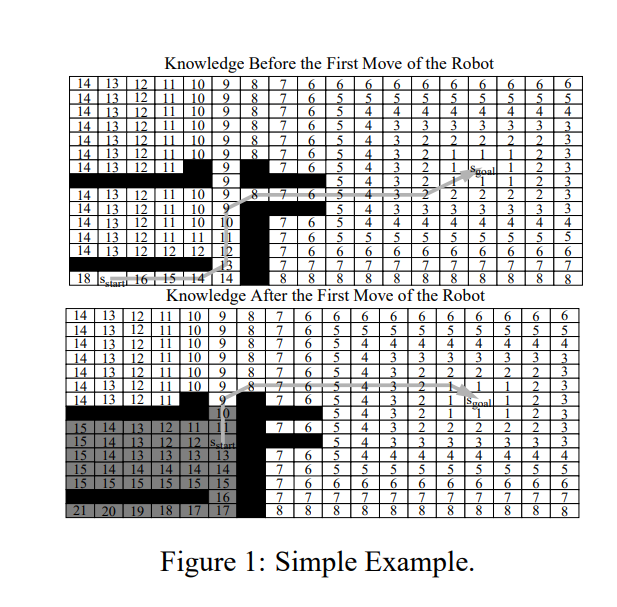
\includegraphics[width=0.8\textwidth]{img/figure1.png}
\end{center}
\newpage
\begin{center}
   \section*{Авторы и история} 
\end{center}
\textbf{Алгоритм D*} — алгоритм поиска кратчайшего пути во взвешенном ориентированном графе, где структура графа неизвестна заранее или постоянно подвергается изменению. Разработан Свеном Кёнигом и Максимом Лихачевым в 2002 году.\\

До того, как в 2002 году был разработан D* Lite, в области поиска пути доминировали другие алгоритмы, такие как A* и алгоритм Дейкстры. D* Lite отличается от этих алгоритмов оптимизации пути двумя основными способами.\\ Во-первых, Дейкстры и A* требуют от пользователя полного знания окружающей среды, поскольку они не предоставляют встроенных функций перепланировки. Это различие означает, что если робот сталкивается с чем-то неизвестным, алгоритмы A* и Дейкстры должны быть полностью перезапущены, чтобы был создан новый путь. С другой стороны, D* Lite быстро пересчитывает только пораженные участки, тем самым значительно сокращая необходимое время обработки. Когда узел обнаруживается как препятствие, стоимость прибытия туда становится бесконечной, и поэтому оценка RHS обновляется до бесконечности.\\Во-вторых, алгоритмы A* и Дейкстры начинаются с генерации пути от начала до конца. D* Lite, с другой стороны, генерирует путь от цели до старта. Это различие полезно для перепланирования, потому что, когда путь необходимо восстановить, требуется меньше изменений при перемещении назад.
\newpage
\begin{center}
   \section*{Описание алгоритма и реализации} 
\end{center}
\subsection*{Алгоритм D*Lite}
\textbf{Постановка задачи}\\
Дан взвешенный ориентированный граф \textbf{\emph{G(V,E)}}.\\
Даны вершины: стартовая вершина \textbf{\emph{f}} и конечная вершина \textbf{\emph{t}}.Требуется после каждого изменения графа \textbf{\emph{G}} обновлять значения функции \textbf{\emph{g(s)}} при поступлении новой информации о графе  \textbf{\emph{G}}

\textbf{Описание}\\
Функция \textbf{\emph{g(s)}} хранит минимальное известное расстояние \textbf{\emph{t}} до \textbf{\emph{s}}.\\ 
Будем поддерживать для каждой вершины два вида смежных с ней вершин:
\begin{itemize}
  \item Обозначим множество $\textbf{\emph{Succ(s)}} \subseteq \textbf{\emph{V}}$ как множество вершин, исходящих из вершины \textbf{\emph{s}}.
  \item Обозначим множество $\textbf{\emph{Pred(s)}} \subseteq \textbf{\emph{V}}$ как множество вершин,входящих в вершину \textbf{\emph{s}}.
\end{itemize}
Возвращает список состояний-преемников для состояния \textbf{\emph{u}} , поскольку это 8-полосный график этот список содержит все соседние ячейки. Если ячейка  не занята, и в этом случае у нее нет преемников.
\begin{lstlisting}[language=C,style=C]
void Dstar::getSucc(state u,list<state> &s) {

    s.clear();
    u.k.first  = -1;
    u.k.second = -1;

    if (occupied(u)) return;
    u.x += 1;
    s.push_front(u);
    u.y += 1;
    s.push_front(u);
    u.x -= 1;
    s.push_front(u);
    u.x -= 1;
    s.push_front(u);
    u.y -= 1;
    s.push_front(u);
    u.y -= 1;
    s.push_front(u);
    u.x += 1;
    s.push_front(u);
    u.x += 1;
    s.push_front(u);
}
\end{lstlisting}

\newpage
Возвращает список всех состояний-предшественников для состояния \textbf{\emph{u}}.
Поскольку это для 8-полосного связного графа, список содержит все соседи для состояния \textbf{\emph{u}}. Занятые соседи не добавляются в список.
\begin{lstlisting}[language=C,style=C]
void Dstar::getPred(state u,list<state> &s) {

    s.clear();
    u.k.first  = -1;
    u.k.second = -1;

    u.x += 1;
    if (!occupied(u)) s.push_front(u);
    u.y += 1;
    if (!occupied(u)) s.push_front(u);
    u.x -= 1;
    if (!occupied(u)) s.push_front(u);
    u.x -= 1;
    if (!occupied(u)) s.push_front(u);
    u.y -= 1;
    if (!occupied(u)) s.push_front(u);
    u.y -= 1;
    if (!occupied(u)) s.push_front(u);
    u.x += 1;
    if (!occupied(u)) s.push_front(u);
    u.x += 1;
    if (!occupied(u)) s.push_front(u);

}
\end{lstlisting}
Функция  0 $\leq$ \textbf{\emph{c(s,s') }} $\leq$ +$\infty$ будет возвращать стоимость ребра \textbf{\emph{(s,s')}}. При этом \textbf{\emph{(s,s')=}}$+\infty$ будет тогда и только тогда, когда ребра \textbf{\emph{(s,s')}} не существует.\\
Возвращает стоимость перехода из состояния a в состояние b. Это может быть либо стоимость переезда из состояния a  в состояние b,мы выбрали первое.
Это также стоимость в 8 сторон
\begin{lstlisting}[language=C,style=C]
double Dstar::cost(state a, state b) {

    int xd = fabs(a.x-b.x);
    int yd = fabs(a.y-b.y);
    double scale = 1;

    if (xd + yd > 1) scale = M_SQRT2;

    if (cellHash.count(a) == 0) return scale*C1;
    return scale*cellHash[a].cost;
}
\end{lstlisting}

\newpage

\paragraph{Определение}
Будем называть \textbf{\emph{rhs}}-значением (значение с правой стороны) такую функцию \textbf{\emph{rhs(s)}}, которая будет возвращать потенциальное минимальное расстояние от \textbf{\emph{f}} до \textbf{\emph{s}} по следующим правилам:
\begin{displaymath}
rhs(s) = \left\{ \begin{array}{ll}
 0 & \textrm{если $s=f$}\\
 min(g(s)+c(s,s'))_{s'\in Pred(s)} & \textrm{иначе}
  \end{array} \right.
\end{displaymath}

\begin{lstlisting}[language=C,style=C]

double Dstar::getRHS(state u) {

    if (u == s_goal) return 0;
    if (cellHash.find(u) == cellHash.end())
        return heuristic(u,s_goal);
    return cellHash[u].rhs;
}
double Dstar::setRHS(state u, double rhs) {

    makeNewCell(u);
    cellHash[u].rhs = rhs;

}
\end{lstlisting}

Так как \textbf{\emph{rhs}}-значение использует минимальное значение из минимальных расстояний от \textbf{\emph{f}} до вершин, входящих в данную вершину \textbf{\emph{s}}, это будет нам давать информацию об оценочном расстоянии от \textbf{\emph{f}} до \textbf{\emph{s}}.
\paragraph{Определение:}
Вершина \textbf{\emph{s}} называется \textbf{\emph{насыщенной}}, если $g(s)=rhs(s)$
\paragraph{Определение:}
Вершина \textbf{\emph{s}} называется \textbf{\emph{переполненной}}, если $g(s)>rhs(s)$
\paragraph{Определение:}
Вершина \textbf{\emph{s}} называется \textbf{\emph{ненасыщенной}}, если $g(s)<rhs(s)$\\
\begin{lstlisting}[language=C,style=C]
//Возвращает значение G для состояния u.
double Dstar::getG(state u) {
    if (cellHash.find(u) == cellHash.end())
        return heuristic(u,s_goal);
    return cellHash[u].g;
}
void Dstar::setG(state u, double g) {

    makeNewCell(u);
    cellHash[u].g = g;
}
\end{lstlisting}
Очевидно, что если все вершины насыщены, то мы можем найти расстояние от стартовой вершины до любой. Такой граф будем называть устойчивым (насыщенным).
\paragraph{Определение:}
Эвристическая функция \textbf{\emph{h(s,s′)}} должна поддерживать неравенство треугольника для всех вершин \textbf{\emph{s,s′,s′′}} $\in V$, т.е. $h(s,s′′)\leq h(s,s′)+h(s′,s′′)$
Так же должно выполняться свойство $(s,s′) \leq c*(s,s′), где c*(s,s′)$, где $c*(s,s′)$ - стоимость перехода по кратчайшему пути из \textbf{\emph{s в s′}}, при этом \textbf{\emph{s и s′}} не должны быть обязательно смежными. \\
Возвращает 8-полосное расстояние между состоянием a и состоянием b.
\begin{lstlisting}[language=C,style=C]
double Dstar::eightCondist(state a, state b) {
    double temp;
    double min = fabs(a.x - b.x);
    double max = fabs(a.y - b.y);
    if (min > max) {
        double temp = min;
        min = max;
        max = temp;
    }
    return ((M_SQRT2-1.0)*min + max);
}
\end{lstlisting}
Само собой разумеется, что эвристика, которую мы используем, - это расстояние в 8 направлениях масштабируется на константу C1 (должно быть установлено значение больше <= min cost).
\begin{lstlisting}[language=C,style=C]
double Dstar::heuristic(state a, state b) {
    return eightCondist(a,b)*C1;
}
\end{lstlisting}

\paragraph{Определение:}
Будем называть ключом вершины такую функцию \textbf{\emph{key(s)}}, которая возвращает вектор из 2-ух значений \textbf{\emph{k1(s)}}, \textbf{\emph{k2(s)}}.
\begin{itemize}
    \item $k1(s)=min(g(s),rhs(s))+h(s,t)$
    \item $k2(s)=min(g(s),rhs(s))$
    \item где \textbf{\emph{s}} - вершина из множества \textbf{\emph{V}}
\end{itemize}

\begin{lstlisting}[language=C,style=C]
state Dstar::calculateKey(state u) {

    double val = fmin(getRHS(u),getG(u));
    u.k.first  = val + heuristic(u,s_start) + k_m;
    u.k.second = val;
    return u;
}
\end{lstlisting}

Если в конце поиска пути $g(t) = + \infty$, путь не найден на данной итерации. Иначе путь найден и "робот" может проследовать по нему.
\paragraph{Примечание:} Так же следует отметить, что функция $init$ не обязана инициализировать абсолютно все вершины перед стартом алгоритма. Это важно, так как на практике число вершин может быть огромным, и только немногие будут пройдены роботом в процессе движения. Так же это дает возможность добавления/удаления ребер без потери устойчивости всех подграфов данного графа.\\
Инициализация d star начинается с координат начала и цели, остальное в соответствии c 
документацией [S. Koenig, 2002]
\newpage
\begin{lstlisting}[language=C,style=C]
void Dstar::init(int sX, int sY, int gX, int gY) {

    cellHash.clear();
    path.clear();
    openHash.clear();
    while(!openList.empty()) openList.pop();

    k_m = 0;

    s_start.x = sX;
    s_start.y = sY;
    s_goal.x  = gX;
    s_goal.y  = gY;

    cellInfo tmp;
    tmp.g = tmp.rhs =  0;
    tmp.cost = C1;

    cellHash[s_goal] = tmp;

    tmp.g = tmp.rhs = heuristic(s_start,s_goal);
    tmp.cost = C1;
    cellHash[s_start] = tmp;
    s_start = calculateKey(s_start);

    s_last = s_start;
}
\end{lstlisting}
\paragraph{Функция (updateVertex):} Если некоторые затраты на ребро изменились,вызывается $UpdateVertex()$, чтобы обновить значения $rhs$ и ключи вершин, потенциально затронутых измененными затратами на ребро, а также их членство в очереди приоритетов, если они становятся \textbf{\emph{насыщенными}} или \textbf{\emph{ненасыщенными}}

\begin{lstlisting}[language=C,style=C]
void Dstar::updateVertex(state u) {
    list<state> s;
    list<state>::iterator i;

    if (u != s_goal) {
        getSucc(u,s);
        double tmp = INFINITY;
        double tmp2;

        for (i=s.begin();i != s.end(); i++) {
            tmp2 = getG(*i) + cost(u,*i);
            if (tmp2 < tmp) tmp = tmp2;
        }
        if (!close(getRHS(u),tmp)) setRHS(u,tmp);
    }
    if (!close(getG(u),getRHS(u))) insert(u);
}
\end{lstlisting}
Обновить позицию робота, это не приведет к принудительному воспроизведению.
\begin{lstlisting}[language=C,style=C]
void Dstar::updateStart(int x, int y) {

    s_start.x = x;
    s_start.y = y;

    k_m += heuristic(s_last,s_start);

    s_start = calculateKey(s_start);
    s_last  = s_start;
}
\end{lstlisting}


\begin{lstlisting}[language=C,style=C]
void Dstar::updateCell(int x, int y, double val) {

    state u;

    u.x = x;
    u.y = y;

    if ((u == s_start) || (u == s_goal)) return;

    makeNewCell(u);
    cellHash[u].cost = val;

    updateVertex(u);
}
\end{lstlisting}

\paragraph{Теорема (О монотонности изменения ключей):}
В течение выполнения функции $ComputeShortestPath$ вершины, взятые из очереди, монотонно не убывают.
\paragraph{Теорема (О необратимой насыщенности):}
Если в функциибыла $ComputeShortestPath$ взята переполненная вершина, то на следующей итерации она станет насыщенной.
\paragraph{Теорема}
После выполнения функции $ComputeShortestPath$ можно восстановить путь из $f в t$. Для этого, начиная с вершины $t$, нужно постоянно передвигаться к такой вершине $s′$, входящей в $t$, чтобы $g(s′)+c(s′,s)$ было минимальным, до тех пора, пока не будет достигнута вершина $f$.
\paragraph{Теорема (Свен Кёниг, Об устойчивой насыщенности вершин):}Функция\\ $ComputeShortestPath$ в данной версии алгоритма расширяет вершину максимум 2 раза, а именно 1 раз, если вершина ненасыщена, и максимум 1 раз, если она переполнена.
\begin{itemize}
\item Прекращаем планирование после нескольких шагов, "maxsteps" мы делаем это
потому что этот алгоритм может планировать вечно, если начало
окруженны препятствиями.
\item Лениво удаляем состояния из открытого списка, чтобы нам никогда не приходилось перебирать его.
\end{itemize}
\begin{lstlisting}[language=C,style=C]
Dstar::Dstar() {
    maxSteps = 80000;  // расширения  узлов
    C1       = 1;      // стоимость невидимой ячейки
}
\end{lstlisting}
\begin{lstlisting}[language=C,style=C]
int Dstar::computeShortestPath() {

    list<state> s;
    list<state>::iterator i;

    if (openList.empty()) return 1;

    int k=0;
    while ((!openList.empty()) &&
           (openList.top() < (s_start = calculateKey(s_start))) ||
           (getRHS(s_start) != getG(s_start))) {

        if (k++ > maxSteps) {
            fprintf(stderr, "At maxsteps\n");
            return -1;
        }

        state u;

        bool test = (getRHS(s_start) != getG(s_start));

        // ленивое удаление
        while(1) {
            if (openList.empty()) return 1;
            u = openList.top();
            openList.pop();

            if (!isValid(u)) continue;
            if (!(u < s_start) && (!test)) return 2;
            break;
        }
        ds_oh::iterator cur = openHash.find(u);
        openHash.erase(cur);

        state k_old = u;

        if (k_old < calculateKey(u)) { // u устарел
            insert(u);
        } else if (getG(u) > getRHS(u)) { // нуждается в обновлении (стало лучше)
            setG(u,getRHS(u));
            getPred(u,s);
            for (i=s.begin();i != s.end(); i++) {
                updateVertex(*i);
            }
        } else {   // g <= rhs, состояние ухудшилось
            setG(u,INFINITY);
            getPred(u,s);
            for (i=s.begin();i != s.end(); i++) {
                updateVertex(*i);
            }
            updateVertex(u);
        }
    }
    return 0;
}
\end{lstlisting}
\paragraph{Открытый хэш и отложенное удаление}
Чтобы ускорить время, необходимое для добавления / удаления / поиска в открытом списке, мы использовали как $stl::priority_queue$, так и $stl ::hash_map$ для хранения состояний.\\Очередь сохраняет состояния в отсортированном порядке, поэтому легко найти следующее лучшее состояние, в то время как хэш используется для быстрого определения того, какие состояния находятся в очереди. Когда ячейка вставляется в $openlist$, она помещается в очередь и помещается в хеш-таблицу. Чтобы проверить, есть ли ячейка в открытом списке, можно просто проверить, есть ли она в хеш-таблице. \\В хэш-таблице также хранится хэш ключа ячеек, поэтому ячейки, которые устарели в очереди, все еще могут быть удалены. Каждый раз, когда ячейка извлекается из очереди, мы проверяем, есть ли она в хэше, если нет, она отбрасывается и выбирается новая.
\\
\\
Возвращает хэш-код ключа для состояния u, который используется для сравнения состояние, которое было обновлено
\begin{lstlisting}[language=C,style=C]
float Dstar::keyHashCode(state u) {
    return (float)(u.k.first + 1193*u.k.second);
}
\end{lstlisting}

Возвращает значение true, если состояние u находится в открытом списке или нет,
проверяя, есть ли оно в хэш-таблице.
\begin{lstlisting}[language=C,style=C]
bool Dstar::isValid(state u) {
    ds_oh::iterator cur = openHash.find(u);
    if (cur == openHash.end()) return false;
    if (!close(keyHashCode(u), cur->second)) return false;
    return true;
}
\end{lstlisting}

Проверяет, есть ли ячейка в хэш-таблице, если нет, то добавляет ее в нее
\begin{lstlisting}[language=C,style=C]
void Dstar::makeNewCell(state u) {
    if (cellHash.find(u) != cellHash.end()) return;
    cellInfo tmp;
    tmp.g       = tmp.rhs = heuristic(u,s_goal);
    tmp.cost    = C1;
    cellHash[u] = tmp;
}
\end{lstlisting}
\newpage
Возвращает значение true, если ячейка занята (недоступна для обхода),в противном случае значение false. непроходимые отмечены стоимостью < 0.
\begin{lstlisting}[language=C,style=C]
bool Dstar::occupied(state u) {

    ds_ch::iterator cur = cellHash.find(u);

    if (cur == cellHash.end()) return false;
    return (cur->second.cost < 0);
}
\end{lstlisting}


\paragraph{Оптимизация евклидова пути }
Получение пути из сгенерированной D* карты затрат обычно выполняется путем запуска с начального узла и выполнения жадного поиска путем расширения последующих узлов с наименьшими затратами до цели. \\
\\
Этот подход может генерировать траекторию, которая начинает двигаться под углом 45 градусов к цели, а не прямо к ней. Это происходит потому, что 8-полосное связное расстояние является приблизительным, и нет никакой разницы между тем, чтобы сначала выполнять все угловые ходы и выполнять все прямые ходы. Чтобы сгенерировать путь, который ближе к истинной наименьшей стоимости, мы добавили простую модификацию в жадный поиск. Когда мы сравниваем затраты со всеми последующими ячейками, мы выбираем ту, которая минимизирует:\\

Евклидова стоимость между состоянием a и состоянием b.
\begin{lstlisting}[language=C,style=C]
double Dstar::trueDist(state a, state b) {

    float x = a.x-b.x;
    float y = a.y-b.y;
    return sqrt(x*x + y*y);

}
\end{lstlisting}
\begin{lstlisting}[language=C,style=C]
bool Dstar::replan() {

    path.clear();
    int res = computeShortestPath();
    FILE *file;
    file=fopen("out.txt","w+t");
    fprintf(file ,"res: %d ols: %d ohs: %d tk: [%f %f] sk: [%f %f] sgr: (%f,%f)\n",res,openList.size(), openHash.size(), openList.top().k.first, openList.top().k.second, s_start.k.first, s_start.k.second, getRHS(s_start), getG(s_start));
    
    if (res < 0) {
        return false;
    }
    list<state> n;
    list<state>::iterator i;

    state cur = s_start;

    if (isinf(getG(s_start))) {
        return false;
    }

    while(cur != s_goal) {

        path.push_back(cur);
        getSucc(cur, n);

        if (n.empty()) {
            return false;
        }

        double cmin = INFINITY;
        double tmin;
        state smin;

        for (i=n.begin(); i!=n.end(); i++) {
            double val  = cost(cur,*i);
            double val2 = trueDist(*i,s_goal) + trueDist(s_start,*i);
            val += getG(*i);

            if (close(val,cmin)) {
                if (tmin > val2) {
                    tmin = val2;
                    cmin = val;
                    smin = *i;
                }
            } else if (val < cmin) {
                tmin = val2;
                cmin = val;
                smin = *i;
            }
        }
        n.clear();
        cur = smin;
    }
    path.push_back(s_goal);
    return true;
}
\end{lstlisting}
\newpage

\paragraph{Main} Функция $Main$ где мы принимаем входные данные.
\begin{itemize}
    \item устанавливаем координаты начала и конца
    \item задаем координаты непроходимой ячейки
    \item задаем стоимость одной из координат ячеки
    \item планируем путь, получаем путь 
    \item изменяем начало на другие координаты
    \item изменяем цель на другие координаты
\end{itemize}

\begin{lstlisting}[language=C,style=C]
int main() {
    Dstar *dstar = new Dstar();
    list<state> mypath;
    FILE *file;
    file = fopen("test1.txt", "r");

    int n1;
    int arr[n1];
    for (int i = 0; i < n1; i++){
        fscanf(file, "%d,", &arr[i] );
    }
    dstar->init(arr[0],arr[1],arr[2],arr[3]); 
    dstar->updateCell(arr[4],arr[5],-1);     
    dstar->updateCell(arr[6],arr[7],42.432); 

    dstar->replan();               
    mypath = dstar->getPath();     

    dstar->updateStart(arr[8],arr[9]);      
    dstar->replan();               
    mypath = dstar->getPath();    

    dstar->updateGoal(arr[10],arr[11]);        
    dstar->replan();               
    mypath = dstar->getPath();     
    fclose(file);
    return 0;
}
\end{lstlisting}
\newpage
\begin{center}
   \section*{Пример работы}
\end{center}
Итерации в функции $ComputeShortestPath$ на исходном графе.
    \begin{center}
        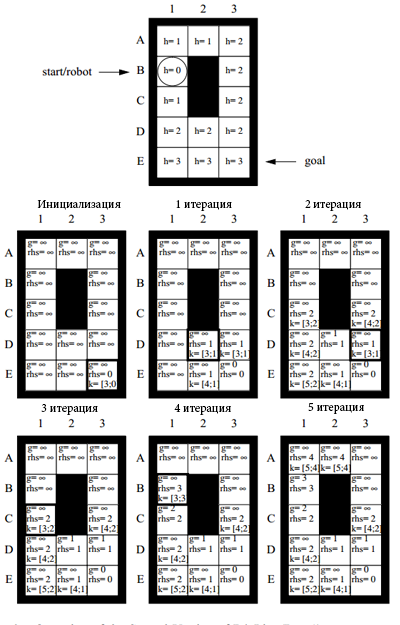
\includegraphics[width=0.45\textwidth]{img/robot.png}
    \end{center}

Итерации в функции $ComputeShortestPath$ после изменения графа. (Второй вызов функции)
    \begin{center}
        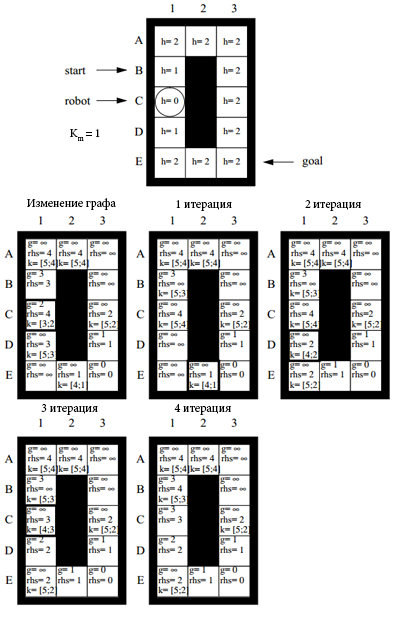
\includegraphics[width=0.45\textwidth]{img/robot2.png}
    \end{center}
\newpage  
\begin{center}
   \section*{Тестирование и анализ производительности}
\end{center}
При измерение времени и работы алгоритма статично выдавало 14ms. При увеличении размера расширения узлов с 8000 до 80 000 000 компилятор стабильно выводил 14ms.
В test1.txt числа не превышали <=10. Тогда создав 8 тестов в зависимости от размера взодящих данных и их увелечения на графике можно увидить как увеличивалось и время выполнения алгоритма.
\begin{center}
        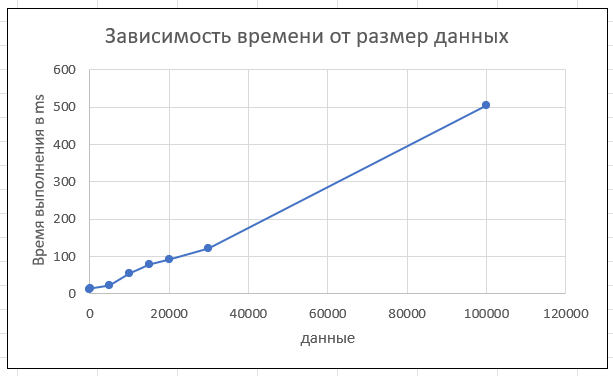
\includegraphics[width=0.7\textwidth]{img/datetime.png}
    \end{center}
\newpage  
\begin{center}
   \section*{Список литературы}
\end{center}

\nocite{*}
\printbibliography
\end{document}
